\documentclass[UTF8]{article}
% \author {Dis\cdot count}
\author {**}

\title {一范数下无容量限制设施选址逆优化问题的求解方法}
\date{}
\usepackage{ctex}
\usepackage{amsmath}

\usepackage{geometry}
\geometry{a4paper,scale=0.8}
\usepackage{graphicx}
\usepackage{amssymb}

\usepackage{algorithm}
\usepackage{algpseudocode}
\usepackage{epsfig}

\usepackage{setspace}
\renewcommand{\baselinestretch}{1.5}

\usepackage{float}
\usepackage{color}%,soul}f
\usepackage{booktabs}
\usepackage{multirow}
\usepackage{xr}

\begin{document}
    \maketitle

\begin{abstract}
逆优化问题是给定一个可行解(值)通过最小化目标函数中参数的改变量使得该可行解(值)成为改变后问题的最优解(值)的问题。对于本是NP-难问题的设施选址问题,其逆优化问题变得更为复杂。研究了使用经典的行生成算法对无容量限制设施选址的逆优化问题进行计算,并给出了得到逆优化问题上下界的启发式方法。两种方法分别基于对子问题的线性松弛求解给出上界和利用邻域搜索的方式给出下界。数值结果表明可行上界得到的结果与最优值差距极小,极大地提高了求解该逆优化问题的效率。所提到的启发式算法还可以推广至有容量设施选址逆优化问题的计算。

% 5. 文章均应附中英文摘要。摘要内容应重点包括4个要素:
% a. 目的-研究的目的和任务,涉及的主题范围;
% b. 方法-研究中使用的方法、理论、手段、条件、材料等;
% c. 结果-研究的结果,数据,被确定的关系,得到的效果、性能等;
% d. 结论-结果的分析、比较、评价、应用,提出的问题,今后的课题,启发,建议,预测等。
\end{abstract}

\qquad \textbf{关键词: 无容量限制设施选址问题、逆优化、行生成算法、启发式算法}

Abstract

The inverse optimization problem is to give a feasible solution (value) by minimizing the change of parameters in the objective function so that the feasible solution (value) becomes optimal after the parameter adjustment. For the facility location problem which is NP-hard, its inverse optimization problem becomes also complex. In this paper, the classical row generation algorithm is used to calculate the inverse optimization problem of uncapacitated facility location, and two heuristic methods are given to get the upper and lower bounds of the inverse optimization problem. The two methods give the upper bound based on the linear relaxation of the subproblem and the lower bound by the local search technique, respectively. The numerical results show that the difference between the feasible upper bound and the optimal value is very small, which greatly improves the efficiency of solving the inverse optimization problem. The proposed heuristic algorithm can also be extended to the calculation of the inverse optimization of the capacitated facility location problem.

Keywords: uncapacitated facility location problem, inverse optimization problem, row generation method, heuristc algorithm

\section{引言}
% 逆优化综述 introduction

逆优化问题最初由 Tarantola (1987) 在地球物理科学中给出了逆优化问题的详细讨论。而在数学规划领域,Burton and Toint (1992, 1994) 研究了在地震层析成像中的最短路径逆优化问题用来预测地震的运动。在之后几年,逆优化在经典运筹学问题中的研究变得更为密集。Zang and Liu (1996) 研究了分配和最小成本流的逆优化问题。Yang et al. (1997) 和 Zhang and Cai (1998) 研究了最小割的逆优化问题。Zhang and Liu (1996, 1999) 讨论了在一范数和无穷范数下的线性规划逆优化的方法。最近,Ahuja and Orlin (2001) 证明了在一范数和无穷范数下,如果原优化问题多项式可解则其标准逆优化问题也是多项式可解的。Heuberger (2004) 给出了逆优化问题较为全面的综述。
% 设施选址问题最初由提出。
最基本的设施选址问题分为无容量限制和有容量限制两种。
由于设施选址问题本身是NP-难的,其逆优化问题很少有人研究。在现实生活中,我们往往需要固定某些设施开启以提供便利。对应到模型中,即给定了开设哪些设施,需要调整成本量达到最小。

本文研究了无容量限制设施选址逆优化(IUFL)问题模型的建立与求解方法。用行生成算法将 IUFL 问题分为主问题和子问题,其中子问题为一般的无容量限制设施选址(UFL)问题。对子问题进行不同的处理方式,可以分别得到 IUFL 问题的上下界。

本文安排如下:第一节给出了 UFL 的定义以及 IUFL问题模型的建立。第二节给出了 IUFL 问题的列生成求解方法。第三节给出了对列生成算法进行改进,得到逆优化问题上下界的启发式算法。第四节给出了 IUFL 逆优化问题的简单示例以及计算结果。第五节给出了对于该逆优化问题延拓以及算法改进的展望。

\section{ UFL 和 IUFL 问题的模型}

设施选址问题通常被提出如下:假设有$m$个设施和$n$个客户。我们希望选择(1)哪些设施要打开,以及(2)哪些打开的设施要用于向哪些客户提供,以便以最低的成本满足某些固定需求。引入以下记号,令$f_i$ 表示开启设施$i$的固定成本,$i \in M, M=\{1,\ldots,m\}$。$r_{ij}$ 表示运输商品从设施$i$到客户$j$的成本,$j \in N, N=\{1,\ldots,n\}$。无容量限制指每个设施可以提供容量$T$是充分大的。

则无容量限制设施选址问题(UFL)定义如下:
\begin{align*}
&\min \sum_{i=1}^n \sum_{j=1}^m r_{ij}u_{ij} + \sum_{i=1}^n f_i v_i \\
\text{s.t.}\quad & \sum_{i=1}^n u_{ij} =1, \forall j \in N  \\
&\sum_{j=1}^m u_{ij}  \leq Tv_i, \forall i \in M \\
& u_{ij} \in \{0,1\}, \quad v_{i} \in \{0,1\}
\end{align*}
用$c=(f,r)$表示成本,并且用更为简洁的方式改写包含足够大容量$T$的上式,得到下式:

\begin{align*}
F(c) = &\min \sum_{i=1}^n \sum_{j=1}^m r_{ij}u_{ij} + \sum_{i=1}^n f_i v_i \\
\text{s.t.}\quad & \sum_{i=1}^n u_{ij} =1, \forall j \in N  \\
& u_{ij}  \leq v_i, \forall i \in M ,\forall j \in N\\
& u_{ij} \in \{0,1\}, \quad v_{i} \in \{0,1\}
\end{align*}

逆优化问题通常分为最优值和最优解问题,当给定原问题的一个可行解$x^0$,通过调整原问题的成本$c$为$d$,使得$x^0$成为调整后问题的最优解。而逆优化最优解问题则是求解在某个范数下使得这个调整量最小的问题。当给定原问题的一个可行值$V_0$,称此时对应的问题为逆优化最优值问题。
为方便以及更贴近现实,我们以一范数为例,即表示调整量之和最小。往往对于设施成本和运输成本调整量的权重并不一样,可以分别设为$w_i^f$ 和$w_{ij}^r$。

无容量限制设施选址的逆优化问题(IUFL)定义如下:
\begin{align*}
&\min_{d} \left\|d-c\right\|_1 \\
\text{s.t.}\quad & dx^0 = F(d) \\
& d \in \mathbb{R}^{mn+m}
\end{align*}

由约束式可以看出,$x^0$需要满足$dx^0 \leq dx^{'}, x^{'} \in \Upsilon$。 其中$\Upsilon$是满足原问题的所有可行解$x^{'}$的集合。对于每一个客户$j \in N$可以被任一设施服务,共有$|M|=m$种选择。因而对于所有客户而言一共会有 $m^n$ 种不同情况。即满足原问题约束条件的可行解有$m^n$个。因此从逆优化的定义出发建立求解模型,上述集合中包含可行解的个数是指数个。事实上,无容量限制设施选址的逆优化问题(IUFL)是NP-难问题。

证明:
假设IUFL问题不是NP-难问题,则可以在多项式时间内对于给定的可行解判断改变量是否为最小。而判断给定的可行解是否为在参数调整之后 UFL 的最优解的复杂度与求解 UFL 问题的复杂度相同。这与 UFL 问题是 NP-难的相矛盾,因而 IUFL 问题是NP-难的。


\section{行生成算法求解}
从设施选址逆优化问题的定义过程中,我们可以看出原优化问题和逆优化问题有着一定的联系,即逆优化中的给定解对应的成本需要小于所有满足原问题约束条件的解对应的成本。行生成算法作为一种有效求解规模较大线性规划问题的方法。我们自然想到行生成算法中子问题即是求解满足原问题约束的,因而行生成算法可以用来求解设施选址的逆优化问题。

原逆优化模型为
\begin{align*}
&\min |c-c_0|  \\
\text{s.t.}\quad & V^0 = cx^0 \leq cx^{'}, x^{'} \in \Upsilon
\end{align*}


为方便显示我们的结果,我们主要考虑最优解问题,而对于最优值问题,给定 $V^0$ 而不是 $x^0$,根据该式 $V^0 = cx^0$ 也可用相同思路求解。

将行生成算法应用于 IUFL 问题,将上式对应的设施和运输部分用 $(f,c)$ 分别表示。
根据Ahuja (2001)在文献中提到在一范数下逆优化问题的处理方法,可以得到 IUFL 问题的主问题为
\begin{align*}
&\min \quad \sum_{i=1}^m w_i^f(a_i+b_i)+\sum_{i=1}^m\sum_{j=1}^n w_{ij}^r(c_{ij}+d_{ij})\\
\text{s.t.}\quad & (a_i-b_i+f_i^0)(v_i^{'}-v_i^{0}) + (c_{ij}-d_{ij}+r_{ij}^0)(u_{ij}^{'}-u_{ij}^{0})  \geq 0 \\
& a_i \geq 0 ,\quad b_i \geq 0,\quad \forall i \in M \\
& c_{ij} \geq 0, \quad d_{ij} \geq 0, \quad \forall i \in M, \forall j \in N\\
& (v_i^{'},u_{ij}^{'}) \in \mathbb{I}
\end{align*}

其中$(v_i^{'},u_{ij}^{'})$属于一个限制集$\mathbb{I}$,集合中的元素由子问题不断生成加入其中。而主问题得到的$(a^{'},b^{'},c^{'},d^{'})$带入到子问题中求解。

子问题如下:

\begin{align*}
T = &\min \quad \sum_{i=1}^m(a_i^{'}-b_i^{'}+f_i^0)(v_i^{'}-v_i^{0})+\sum_{i=1}^m\sum_{j=1}^n(c_{ij}^{'}-d_{ij}^{'}+r_{ij}^0)(u_{ij}^{'}-u_{ij}^{0}) \\
\text{s.t.}\quad & \sum_{i=1}^m u_{ij}^{'} =1, \quad \forall j\in N \\
& u_{ij}^{'} \leq v_{i}^{'}, \quad \forall i \in M, \forall j \in N \\
& u_{ij}^{'} \geq 0, \quad \forall i \in M, \forall j \in N \\
&u_{ij}^{'} \in \{0,1\} ,\quad v_{i}^{'} \in \{0,1\}
\end{align*}

子问题求出得到 $(v^{'*},u^{'*})$, 如果目标函数值小于0,将得到的 $(v^{'*},u^{'*})$ 加入到主问题的限制集中。如果目标函数值不小于0,程序结束。
注意到子问题实际上是无容量限制设施选址的原问题,因此该设施选址的逆问题复杂度要大于原问题,也是NP-难问题。

求解 IUFL 问题的行生成算法详细步骤如下:

输入:1) 可行解:$x^0=(v_i^0,u_{ij}^0)$; 2)原设施成本:$c^0=(f_i^0,r_{ij}^0)$;

输出:1)最优解 $(a^{*},b^{*},c^{*},d^{*})$;
2) 最小的总成本改变量为
$\sum_{i=1}^m(a^{*}_i+b^{*}_i)+\sum_{i=1}^m\sum_{j=1}^n(c^{*}_{ij}+d^{*}_{ij})$ ;
3) 对应原成本的改变量为 $f_i-f_i^0 = a^{*}_i-b^{*}_i,r_{ij}-r_{ij}^0=c^{*}_{ij}-d^{*}_{ij}$.

初始化:初始限制集包含对于原问题的可行解即可。为方便且不再重新生成可行解,可取初始限制集为给定的可行解即 $\mathbb{I} = \{(v_i^0,u_{ij}^0)\} $。

步骤 1:求解此时的主问题得到最优解 $(a^{'},b^{'},c^{'},d^{'})$.

步骤 2:将步骤 1得到的最优解 $(a^{'},b^{'},c^{'},d^{'})$带入到子问题中,求解子问题这一整数规划得到最优解 $x^{'*}=(v^{'*},u^{'*})$ 和目标函数值$T$.

步骤 3:如果目标函数值$T< 0$, 将得到的 $x^{'*}$ 加入到限制集中$\mathbb{I} = \mathbb{I} \cup \{x^{'*}\}$,回到步骤 1,重新求解主问题;  如果目标函数值$T\geq 0$,则结束算法。此时得到最优解$(a^{*},b^{*},c^{*},d^{*})$。


\section{启发式算法得到上下界}

由上述的行生成方法,我们可以知道要求得逆优化的最优解就需要得到尽可能精确的主问题的限制集,即主问题中的限制条件。由于主问题的限制集是由子问题不断生成得到的,可以看出行生成方法的核心是子问题的效率,即子问题求解越精确,逆优化的最优解越精确。但由于子问题是设施选址的原问题,因而可以通过对子问题进行松弛,牺牲一定求解精度的情况下简化求解过程。

当对子问题进行如下几种处理方法时,我们可以相应得到行生成方法的几点推论:

\textbf{处理方法 1}:严格求解子问题,即求解上式

推论 1. 当严格求解子问题时,循环结束时此时得到IUFL问题的最优解。

说明:由于子问题是不断从 UFL 问题的约束中筛选出满足条件的解 $(v^{'*},u^{'*})$, 严格求解子问题直到循环结束,筛选出来的解集 $\mathbb{I}$ 满足UFL所有的约束条件,根据逆优化问题的定义,根据此时的解集求解主问题得到的即是逆优化问题的最优解。

\textbf{处理方法 2}:严格求解子问题但设定一定的循环次数

推论 2. 严格求解子问题时,设定一定的循环次数,此时求解得到 IUFL 问题的下界。

说明:当循环一定次数时,此时子问题得到的限制集较最优时少,因而主问题的约束条件较最优时少。实际上减少了一些所必须的约束,此时主问题求解得到的目标函数值小于最优值,因而得到逆优化问题的下界。

\textbf{处理方法 3}: 对子问题利用邻域搜索得到启发式整数解。

推论 3. 对子问题利用邻域搜索方法求解,此时求解得到 IUFL 问题的下界。

说明:对于子问题给定一个可行解,利用邻域搜索的方法得到较优的整数解作为返回值。邻域搜索采用基本的本地搜索方法(Ghosh D.),即对于当前给定解采用增加,交换和减少的方式得到局部最优整数解。

由于行生成算法结束的条件是比较给定解对应的成本和原问题松弛求解出的最小成本 $min_{LP}$ 的大小. 由于 $min_{LP}$ 求出来的是上界,所以当 $min_{LP}$ 松弛效果不好时,就会导致提前结束。

下面对邻域搜索的三种方式进行说明。设此时未开启设施的数量为 $p$,开启设施的数量为$m-p$。

增加,即对于当前未开启的设施中开启一个设施,作为一个增加邻域,共有$p$个邻域。

交换,即对于当前未开启的设施中开启一个设施,在开启的设施中关闭一个设施,作为一个交换邻域,共有$p(m-p)$个邻域。

减少,即对于当前开启的设施中关闭一个设施,作为一个减少邻域,共有$(m-p)$个邻域。

在一次求解过程中,对于三种方式得到的邻域解对应的成本进行比较,取最小值求得对应的局部最优解。将当前给定解转移到得到的局部最优解,返回该局部最优解到主问题,再进行下一次求解。

求解 UFL 下界的启发式算法详细步骤如下:

输入:1) 可行解:$x^0=(v_i^0,u_{ij}^0)$; 2)原设施成本:$c^0=(f_i^0,r_{ij}^0)$;

输出:1)最优解 $(a^{*},b^{*},c^{*},d^{*})$;
2) 最小的总成本改变量为
$\sum_{i=1}^m(a^{*}_i+b^{*}_i)+\sum_{i=1}^m\sum_{j=1}^n(c^{*}_{ij}+d^{*}_{ij})$ ;
3) 对应原成本的改变量为 $f_i-f_i^0 = a^{*}_i-b^{*}_i,r_{ij}-r_{ij}^0=c^{*}_{ij}-d^{*}_{ij}$.

初始化:初始限制集包含对于原问题的可行解即可。为方便且不再重新生成可行解,可取初始限制集为给定的可行解即 $\mathbb{I} = \{(v_i^0,u_{ij}^0)\} $。

步骤 1:求解此时的主问题得到最优解 $(a^{'},b^{'},c^{'},d^{'})$.

步骤 2:将步骤 1得到的最优解 $(a^{'},b^{'},c^{'},d^{'})$带入到子问题中,给定子问题初始解为$ $, 这一整数规划得到最优解 $x^{'*}=(v^{'*},u^{'*})$,和目标函数值$T$.

步骤 3:如果目标函数值$T< 0$, 将得到的 $x^{'*}$ 加入到限制集中$\mathbb{I} = \mathbb{I} \cup x^{'*}$,回到步骤 1,重新求解主问题;  如果目标函数值$T\geq 0$,则结束算法。此时得到最优解$(a^{*},b^{*},c^{*},d^{*})$。


\textbf{处理方法 4}:直接对子问题进行线性松弛求解

推论 4. 将无容量限制设施选址的子问题松弛得到线性规划问题,依然按照之前的步骤求解则可以得到对应逆优化问题的上界。

说明:当对子问题的整数规划问题进行线性松弛时,可以得到非整数解。此时会得到子问题的下界,对应的主问题会得到约束更为严格的限制集。主问题对应的可行域变小,使得最终得到的结果大于最优解,此时得到逆优化问题的上界。

此时对应的子问题模型变为:

\begin{align*}
T = &\min \quad \sum_{i=1}^m(a_i^{'}-b_i^{'}+f_i^0)(v_i^{'}-v_i^{0})+\sum_{i=1}^m\sum_{j=1}^n(c_{ij}^{'}-d_{ij}^{'}+r_{ij}^0)(u_{ij}^{'}-u_{ij}^{0}) \\
\text{s.t.}\quad & \sum_{i=1}^m u_{ij}^{'} =1, \quad \forall j\in N \\
& u_{ij}^{'} \leq v_{i}^{'}, \quad \forall i \in M, \forall j \in N \\
& u_{ij}^{'} \geq 0, \quad \forall i \in M, \forall j \in N \\
& 0 \leq u_{ij}^{'} \leq 1 ,\quad 0 \leq v_{i}^{'} \leq 1
\end{align*}


% \subsection{启发式得到上界}
% 有学者利用合作博弈的思想和锥优化的方法得到了一种无容量限制设施选址逆优化的启发式算法,我们将主要阐述他的方法并且显示了我们得到上界的启发式算法与之等价,从而可以得到我们的启发式算法在多项式时间内得到较为优异的结果。
%
% 在2010文章中,Letchford 定义了关于设施选址问题的最小整数(Interger Minimization)博弈,并且给出了无容量限制设施选址问题的锥可行域在$x$上的投影。
% \[
% \mathbb{C}_{\mathrm{UFL}}^{x}=\left\{(v, u) \in \mathbb{R}^{m+m v}: \sum_{i \in M} u_{i j}=1, \forall j \in V, v_{i}-u_{i j} \geq 0, \forall i \in M, \forall j \in V, u_{i j} \geq 0, \forall i \in M, \forall j \in V\right\}
% \]
% 事实上上述可行域只是将原 UFL 的整数条件进行了松弛
%
% Liu 利用该可行域和锥优化的方法对UFL的逆优化问题得到了如下的启发式算法
% \begin{equation}
% \begin{aligned}
% &\min \sum_{i \in M} \left(\tau_{i}^{f}+\eta_{i}^{f}\right)+\sum_{i \in M} \sum_{j \in V} \left(\tau_{i j}^r+\eta_{i j}^{r}\right) \\
% \text{s.t.} \quad &\sum_{j \in V} \pi_{j} \geq \nu_{\mathrm{UFL}}, \\
% &\sum_{j \in V} \varrho_{i j}=\bar{f}_{i}, \forall i \in M, \\
% &\pi_{j}-\varrho_{i j}+\zeta_{i j}=\bar{r}_{i j}, \quad \forall i \in M, \forall j \in V, \\
% &\sum_{i \in M} \bar{f}_{i} v_{i}^{0}+\sum_{i \in M} \sum_{j \in V} \bar{r}_{i j} u_{i j}^{0}=\nu_{\mathrm{UFL}}, \\
% & \tau_{i}^{f}-\eta_{i}^{f}=\bar{f}_{i}-f_{i}^{*}, \forall i \in M \quad \tau_{i j}^{r}-\eta_{i j}^{r}=\bar{r}_{i j}-r_{i j}, \forall i \in M, \forall j \in V, \\
% & \varrho_{i j} \geq 0, \zeta_{i j} \geq 0, \forall i \in M, \forall j \in V. \\
% \end{aligned}
% \end{equation}
% % \nu_{\mathrm{UFL} 1} \leq \nu_{\mathrm{UFL}} \leq \nu_{\mathrm{UFL} 2},
% 其中$\bar{f}_{i}$和$\bar{r}_{ij}$ 为改变后的开启设施成本和运输成本。相对应的,$f_{i}$和$r_{ij}$ 为改变前的成本。
% $\pi_{j},\varrho_{i j},\zeta_{i j}$分别为原UFL约束
% \begin{equation*}
% \sum_{i \in M} u_{ij} = 1,
% v_i - u_{ij} \geq 0,
% u_{ij} \geq 0
% \end{equation*}
% 对应的对偶变量。 \par
% $v_{i}^{0},u_{i j}^{0}$ 则对应于给定的可行解使之成为改变成本后的最优解。
% $\nu_{\mathrm{UFL}}$ 是原UFL的最优值。
%
% $\tau_{i}^{f},\eta_{i}^{f},\tau_{i j}^r,\eta_{i j}^{r}$ 则对应于求解范数一下引入的变量。 \par
%
%
% 这部分gap很小,实际上对应到(integrality gap)

% \section{求解lower bound 的一些方法}
%
% \subsection{利用邻域的想法}
%
% 有如下约束限制可以帮助给定的可行解在一定范围内是最优的 \\
% 约束一(横向移动):对于给定的可行解(0-1)  对应的 $r_{ij}=1$ 需要小于其他所有 $r_{ij} = 0$ \\
% 约束二(0-1纵向移动):f 中为0 的部分 需要确保  $f_i +\min_i r_{ij} \geq \min r_{ij}$ \\
% 约束三(纵向移动):对于仅有一个 $r_ij=1$ 的行,考虑$r_{ij}+f_i \leq \min_j r_{jj}$ \\
% 约束四:考虑$f_i = 1$中 $r_{ij} =1$ 个数大于1的行 则有$\max f_i+ \sum r_{ij} \leq \min \text{对应列的} r_{ij}$

\section{示例及计算结果}

\subsection{简单的例子}

举出一个简单的例子用来说明逆优化的效果。
% 在Matlab中将图像imshow()一下,然后对figure用另存为eps,这个也能凑活用。
\begin{figure}[h]
\centering
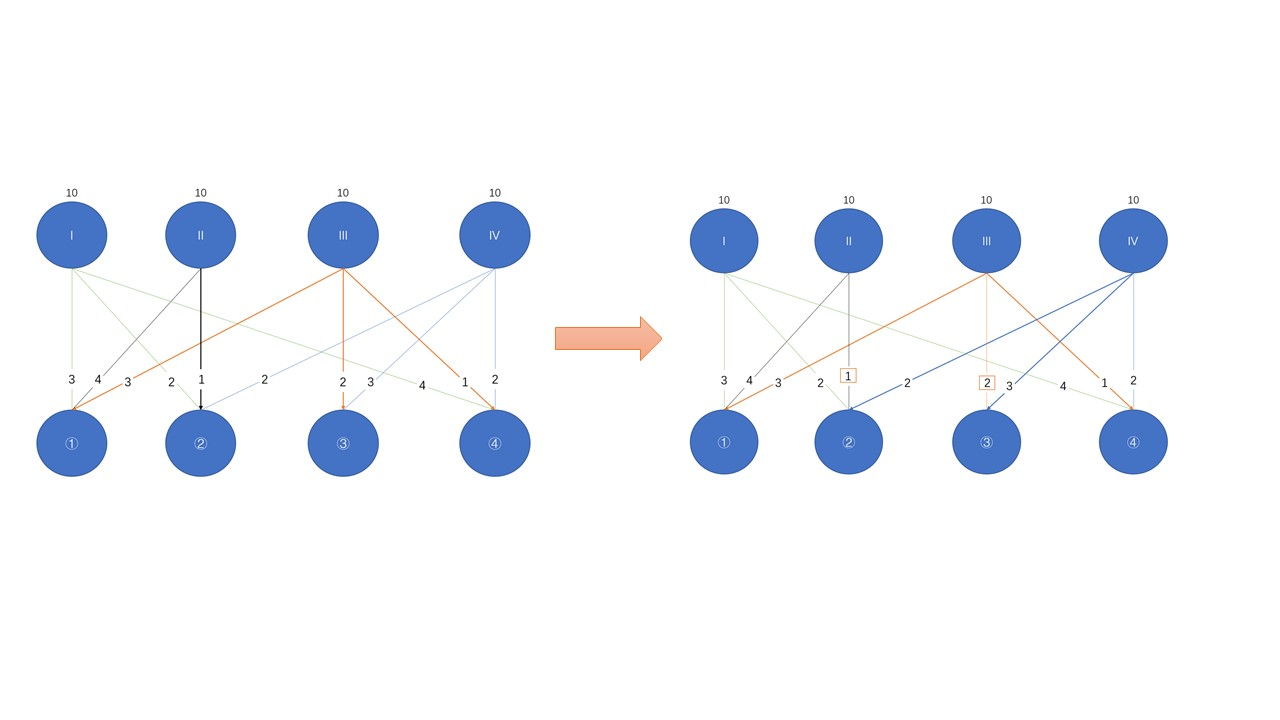
\includegraphics[width=1\textwidth]{Graph}
\caption{例子说明}
\end{figure}

如上图所示,$\uppercase\expandafter{\romannumeral1},\uppercase\expandafter{\romannumeral2},\uppercase\expandafter{\romannumeral3},\uppercase\expandafter{\romannumeral4}$ 为设施编号,每个设施开启成本为$10$。
$a,b,c,d$ 为顾客编号,设施与顾客有连线表示该顾客可以被相应设施服务,连线上的数字表示对应的运输成本。细线表示该问题所有可行的服务连线,左侧图中粗线表示服务最优解连线。右侧图中粗线则表示给定的可行解服务连线。

相应的设施开启成本和运输成本为:

$$
\begin{gathered}
f_i^0 = \begin{pmatrix} 10 \\ 10 \\ 10 \\ 10  \end{pmatrix},
\quad
r_{ij}^0 = \begin{pmatrix} 3 & 2 & M & 4 \\
                          4 & 1 & M & M \\
                          3 & M & 2 & 1 \\
                          M & 2 & 3 & 2 \\
            \end{pmatrix}
\end{gathered}
$$
其中 $M$ 表示一个足够大的数。
能够看出,最优解如左图所示,即为开设设施$\uppercase\expandafter{\romannumeral2}$服务顾客$b$,以及开设设施$\uppercase\expandafter{\romannumeral3}$服务顾客$a,c,d$,对应的最优成本为27。而当给定可行解如右图所示,即为开设设施$\uppercase\expandafter{\romannumeral3}$服务顾客$a,d$,以及开设设施$\uppercase\expandafter{\romannumeral4}$服务顾客$b,c$时,对应的成本为29。需要改变方框中的运输成本使得给定的可行解成为改变成本后的最优解,即将方框中1改为2,方框中2改为3。此时最小改变量为2,可以使得给定的可行解成为改变成本后问题的最优解。

\subsection{计算结果}

本文使用 Windows 10 操作系统,内存 8 GB 处理器为 Intel Core i7-8700 的 PC 电脑上进行了所有的数值实验。所有算法均通过 Matlab R2019a 调用 Gurobi 求解器去实现。
按照规模 $(m,n)$ 大小以及设施成本与运输成本之间关系,在数值实验中,我们对于12种不同规模随机生成了对应规模下50种可能的实例。
% 这里写表格
(m,n)= (20,20) (30,30) (40,40) (50,50)

       (20,40) (30,60) (40,80) (50,100)

       (20,60) (30,90) (40,120) (50,150)

其中设施的启动成本取值范围如下:整数解 $f_i=[1,100]$ ;
    运输成本取值范围如下:$r_{ij}= [1,100],[100,200]$ 。

为方便起见,在接下来的计算中取 $w^f=1,w^r=1$。在实际不能改变设施成本时,可以设置相应的权重$w^f=\infty$。

当最优改变量不为 0 时,我们采用相对百分值(上界改变量-最优改变量)/最优改变量($\%$)的方式来比较 gap 的大小。
同时,当给定可行解刚好是最优解时,此时最优改变量为 0,我们采用绝对值即总的改变量来衡量 gap 或者利用总成本改变量除以总的成本。

结果如下:
{\small\begin{table}[h!]

\centerline{\small{\heiti\bf Table1}  给定可行解非最优解时,IUFL问题的计算结果}
\vskip 2mm
\centering
\begin{tabular}{lccccccc}
    \shline
规模&LB1 &LB2&UB  &OS & GAP1 & GAP2 & GAP3\\
    \hline
$(20,20)-1$ & 0 & 0 & 0  & 0 & 0\\
$(30,30)-1$ & 0 & 0   & 0  & 0 \\
$(40,40)-1$ & 0 & 0 & 0  & 0 \\
$(50,50)-1$ & 0 & 0   & 0  & 0 \\
$(20,40)-1$ & 0 & 0   & 0  & 0 \\
$(30,60)-1$ & 0 & 0   & 0  & 0 \\
$(40,80)-1$ & 0 & 0   & 0  & 0 \\
$(50,100)-1$ & 0 & 0   & 0  & 0 \\
$(20,60)-1$ & 0 & 0   & 0  & 0 \\
$(30,90)-1$ & 0 & 0   & 0  & 0 \\
$(40,120)-1$ & 0 & 0   & 0  & 0 \\
$(50,150)-1$ & 0 & 0   & 0  & 0 \\
$(20,20)-2$ & 0 & 0 & 0  & 0 \\
$(30,30)-2$ & 0 & 0   & 0  & 0 \\
$(40,40)-2$ & 0 & 0 & 0  & 0 \\
$(50,50)-2$ & 0 & 0   & 0  & 0 \\
$(20,40)-2$ & 0 & 0   & 0  & 0 \\
$(30,60)-2$ & 0 & 0   & 0  & 0 \\
$(40,80)-2$ & 0 & 0   & 0  & 0 \\
$(50,100)-2$ & 0 & 0   & 0  & 0 \\
$(20,60)-2$ & 0 & 0   & 0  & 0 \\
$(30,90)-2$ & 0 & 0   & 0  & 0 \\
$(40,120)-2$ & 0 & 0   & 0  & 0 \\
$(50,150)-2$ & 0 & 0   & 0  & 0 \\
   \shline
 \end{tabular}
 \end{table}}

Table2 给出了当给定可行解为最优解时,IUFL问题的计算结果。由定义可知,此时最优值始终为0。此时GAP计算方式改为 (启发式解-最优值)。
 {\small\begin{table}[h!]
 \centerline{\small{\heiti\bf Table2}  给定可行解为最优解时,IUFL问题的计算结果}
 \vskip 2mm
 \centering
 \begin{tabular}{lccccccc}
     \shline
 规模&LB1 &LB2&UB  &OS & GAP1 & GAP2 & GAP3\\
     \hline
 $(20,20)-1$ & 0 & 0 & 0  & 0 & 0\\
 $(30,30)-1$ & 0 & 0   & 0  & 0 \\
 $(40,40)-1$ & 0 & 0 & 0  & 0 \\
 $(50,50)-1$ & 0 & 0   & 0  & 0 \\
 $(20,40)-1$ & 0 & 0   & 0  & 0 \\
 $(30,60)-1$ & 0 & 0   & 0  & 0 \\
 $(40,80)-1$ & 0 & 0   & 0  & 0 \\
 $(50,100)-1$ & 0 & 0   & 0  & 0 \\
 $(20,60)-1$ & 0 & 0   & 0  & 0 \\
 $(30,90)-1$ & 0 & 0   & 0  & 0 \\
 $(40,120)-1$ & 0 & 0   & 0  & 0 \\
 $(50,150)-1$ & 0 & 0   & 0  & 0 \\
 $(20,20)-2$ & 0 & 0 & 0  & 0 \\
 $(30,30)-2$ & 0 & 0   & 0  & 0 \\
 $(40,40)-2$ & 0 & 0 & 0  & 0 \\
 $(50,50)-2$ & 0 & 0   & 0  & 0 \\
 $(20,40)-2$ & 0 & 0   & 0  & 0 \\
 $(30,60)-2$ & 0 & 0   & 0  & 0 \\
 $(40,80)-2$ & 0 & 0   & 0  & 0 \\
 $(50,100)-2$ & 0 & 0   & 0  & 0 \\
 $(20,60)-2$ & 0 & 0   & 0  & 0 \\
 $(30,90)-2$ & 0 & 0   & 0  & 0 \\
 $(40,120)-2$ & 0 & 0   & 0  & 0 \\
 $(50,150)-2$ & 0 & 0   & 0  & 0 \\
    \shline
  \end{tabular}
  \end{table}}

在表中,$(m,n)-1$ 表示 IUFL 问题的规模。例如 $(20,40)-1$ 表示20个设施和 40个客户;$1 $表示$f_i=[1,100],r_{ij}= [1,100]$;$2 $表示$f_i=[1,100],r_{ij}= [100,200]$。

LB1 表示使用迭代次数得到的 P 的下界。
LB2 表示使用邻域搜索得到的 P 的下界。
UB  表示使用线性松弛的方法得到的 P 的上界。
OS 表示严格求解子问题时得到的逆优化问题的最优值。
在Table1中GAP计算方法为百分比法,在Table2中GAP计算方法为绝对值法。
GAP1 表示LB1与OS之间的gap,GAP2 表示LB2与OS之间的gap,GAP3 表示UB与OS之间的gap。
表中所有的结果是一个规模中产生的50个实例的平均值。

计算结果表明,问题的规模$(m,n)$以及设施开设成本$f_i$和运输成本$r_{ij}$的大小关系不影响gap。

\section{有容量限制}

更进一步,令$d_j$ 表示客户$j$的需求,并且假设每一个设施有一个最大输出限制,令$k_i$表示设施$i$能够生产出的最大商品量,即表示设施$i$的容量。

类似的,有容量限制的设施选址问题定义如下:
\begin{align*}
&\min \sum_{i=1}^n \sum_{j=1}^m c_{ij}u_{ij} + \sum_{i=1}^n f_i v_i \\
\text{s.t.}& \sum_{i=1}^n u_{ij} =1, \forall j \in N  \\
&\sum_{j=1}^m d_j u_{ij}  \leq k_iv_i, \forall i \in M \\
& 0 \leq u_{ij} \leq 1,\forall j \in N, \forall i \in M \\
& v_{i} \in \{0,1\}, \forall i \in M
\end{align*}

我们同样可以使用上述提到的行生成算法和启发式方法得到最优解。在此不再赘述。

% \subsection{启发式得到上界}
% 尽管原文章中并未提到有容量限制的设施选址逆优化问题的启发式算法,但我们依然沿用2010中定义以及2019中提到的锥优化方法。
%
% 对于有容量限制的设施选址逆优化问题,需要添加一个约束,此时尽管
% \begin{eqation}
%   \sum_j d_j u_{ij} \leq k_i v_i,i\in M
% \end{eqation}。
% 同样利用锥优化的方法,添加对应上述约束的对偶变量$t$,我们可以得到有容量限制的设施选址问题的启发式算法
%
% \begin{equation}
% \begin{aligned}
% &\min \sum_{i \in M} \left(\tau_{i}^{f}+\eta_{i}^{f}\right)+\sum_{i \in M} \sum_{j \in V} \left(\tau_{i j}^r+\eta_{i j}^{r}\right) \\
% \text{s.t.} \quad &\sum_{j \in V} \pi_{j} \geq \nu_{\mathrm{UFL}}, \\
% &k_it_i+\sum_{j \in V} \varrho_{i j}=\bar{f}_{i}, \forall i \in M, \\
% &\pi_{j}-\varrho_{i j}+\zeta_{i j}-d_jt_i=\bar{r}_{i j}, \quad \forall i \in M, \forall j \in V, \\
% &\sum_{i \in M} \bar{f}_{i} v_{i}^{0}+\sum_{i \in M} \sum_{j \in V} \bar{r}_{i j} u_{i j}^{0}=\nu_{\mathrm{UFL}}, \\
% & \tau_{i}^{f}-\eta_{i}^{f}=\bar{f}_{i}-f_{i}, \forall i \in M \quad \tau_{i j}^{r}-\eta_{i j}^{r}=\bar{r}_{i j}-r_{i j}, \forall i \in M, \forall j \in V, \\
% &\nu_{\mathrm{UFL} 1} \leq \nu_{\mathrm{UFL}} \leq \nu_{\mathrm{UFL} 2}, \varrho_{i j} \geq 0, \zeta_{i j} \geq 0, \forall i \in M, \forall j \in V. \\
% \end{aligned}
% \end{equation}
% 注意这部分 可以通过改变 需求和供给 的大小来退化得到 无容量限制

% 对于行生成的方法,实际上是限制集的选取的问题,限制集越接近

\section{结论与展望}

本文针对无容量限制的设施选址逆优化问题进行了建模分析,提出了使用行生成算法得到最优解以及通过对整数规划进行线性松弛而得到启发式方法。分析表明对于行生成算法中的子问题采取不同的计算方法可以分别得到逆优化问题的最优解以及解的上下界。数值实验结果说明了得到的启发式算法在上界上的优异表现,而在牺牲一定计算资源的情况下,下界也可以得到较为不错的结果。这些结果充分说明了该启发式算法的有效性。
实际上,尽管上界非常接近最优值,但下界的结果可以进一步优化改进。由于子问题是设施选址的原问题,可以将求解设施选址更为高效的近似算法用于其中,从而提高下界解的质量。子问题是最具有优化空间的地方,可以结合启发式算法一次找出多个目标函数小于0的解,并一次性全部加入主问题中进行求解。
同时,尽管本文只提到了无容量限制的设施选址逆优化问题,但提出的算法也可以用在有容量限制的设施选址逆优化问题中。


% 优秀的人总是要比别人多努力一点

\section*{参考文献}

[1] Ghosh D. Neighborhood search heuristics for the uncapacitated facility location problem[J]. European Journal of Operational Research, 2003, 150(1): 150-162.

[2] Tarantola,A.1987.InverseProblemTheory:MethodsforDataFitting and Model Parameter Estimation. Elsevier, Amsterdam.

[3] Burton, D., Ph. L. Toint. 1992. On an instance of the inverse shortest paths problem. Math. Programming 53 45–61.

[4] Zhang, Z. Liu. 1996. Calculating some inverse linear programming problem. J. Comput. Appl. Math. 72 261–273.

[5] Yang, C., J. Zhang, Z. Ma. 1997. Inverse maximum flow and minimum cut problem. Optimization 40 147–170.

[6] Zhang, J., Liu, Z.: Calculating some inverse linear programming problems. J. Comput.Appl. Math. 72, 261–273 (1996)

[7] Zhang,J.,Liu,Z.:Afurtherstudyoninverselinearprogrammingproblems.J.Comput.Appl.Math.106, 345–359 (1999)

[8] Ahuja, R.K., Orlin, J.B.: Inverse optimization. Oper. Res. 49, 771–783 (2001)

[9] Heuberger,C.:Inversecombinatorialoptimization:Asurveyonproblems,methods,andresults.Toappear in Journal of Combinatorial Optimization, 2004


\end{document}
